\section{Experimental evaluation} \label{sec:eval}

In the experimental evaluation, we show that Hypermnesia achieves eventual consistency.
We also evaluate the performance of Hypermnesia in terms of its throughput and latency,
compared against the standard Mnesia, as well as PostgreSQL\footnote{} and MongoDB\footnote{}.

We start by introducing new tests to ensure
the correctness of the system (\cref{sec:eval correctness}), and then outline
the benchmarking approach (\cref{sec:eval benchmarks}), before performing 
measurements on a cluster of distributed physical machines in terms of
time (\cref{sec:eval benchmarks}) and space (\cref{sec:eval space}).
We also include a comparison of Hypermnesia against other popular 
databases (\cref{subsec:eval other db}).
This is followed by an examination of the fault tolerance properties of Hypermnesia
(\cref{sec:eval fault tolerance}).
We conclude the evaluation with a discussion on the API usability of 
Hypermnesia (\cref{sec:eval api}).

\subsection{Setup}

The experiments are performed on:
\begin{enumerate*}[(a)]
  \item a single physical machine with multiple Erlang VMs connected via the loopback 
  interface, mainly used for correctness testing and some simple experiments;
  \item multiple physical machines inside a data centre connected via ethernet
  switches, used for more extensive benchmarking.
\end{enumerate*}

The single physical machine has an AMD 12-Core Processor and 16GiB DDR4 memory. 
It runs the Ubuntu 22.04.2 LTS Operating System. The cluster consists
of 10 machines, each has an Intel(R) Xeon(R) CPU with 6 cores and 64GiB memory.
They all run the Ubuntu 20.04.4 LTS Operating System. More details on the test-bed
setup can be found in~\cref{appendix:eval setup}.


To evaluate Hypermnesia against MongoDB and PostgreSQL, we use Kubernetes to simplify
the deployment process. For MongoDB, the MongoDB enterprise operator\footnote{} is used
to setup a Replica Set of MongoDB instances. MongoDB's replication is asynchronous,
similar to the \verb|async_ec| access context of Hypermnesia. PostgreSQL is deployed 
with the Bitnami's \texttt{postgresql-ha} helm chart, which uses PostgreSQL's builtin
streaming replication for duplicating data. This process is also asynchronous, which
is desirable for our purposes.


\subsection{Correctness} \label{sec:eval correctness}

The first question of whether eventual consistency is possible in 
Mnesia (\cref{itm:question ec possible} in~\cref{sec:intro motivation}) is
concerned with the design and correctness of the implementation, therefore
correctness testing is performed.
The Mnesia source code has a regression test suite with about 5000 tests, 
covering various aspects of the correctness such as transaction, 
dirty operations, storage engine, etc. They are
run against the additional code introduced by Hypermnesia. These
mostly serve as tests for backwards compatibility, since there is currently no 
test that simulates network partitions, nor tests targeting the new eventually 
consistent API\@.

To cover the new \acrshort{ec} API, the suite is extended by
adding the following tests:

\begin{enumerate}
  \item Unit tests on the behaviour of the \acrshort{awset}
  and causal delivery, such as testing, among others, whether the addition of an 
  element is reflected in a subsequent read.
  \item Unit Tests on database features such as index reads.
  \item Integration tests for simulating network partitions, including multiple 
  cases of concurrent addition and deletion.
\end{enumerate}

There are about 20 new tests written to cover the new API. 
Both unit tests and integration tests generally follow the pattern of the Erlang
EUnit and Common Test framework~\cite{ericssonab2023eunit,ericssonab2023ct},
respecting the existing test suite structure. The network partition is simulated with
a custom Erlang distribution protocol~\cite{ericssonab2023erldistro}, 
developed by RabbitMQ for their integration testing~\cite{rabbitmq2022inet_tcp_proxy}.

Hypermnesia passes all of the tests mentioned above, and the output
log of the tests is included in~\cref{appendix:test output}.

\subsection{Benchmarking} \label{sec:eval benchmarks}


The second question (\cref{itm:question ec overhead} in~\cref{sec:intro motivation}) 
is concerned with the efficiency of the \acrlong{ec} \acrshort{api} in Hypermnesia. 
To answer this question, benchmarking is performed on the Hypermnesia codebase.
The original Mnesia repository has a built-in benchmarking suite for transactions. 
Briefly, this benchmark is a
simulation of workloads where Mnesia tables are used to store session data of,
for example, users logging into a website. There are four stages in this benchmark:

\begin{description}
  \item[population] initialises tables with randomly generated data.
  \item[warmup] performs operations to bring data from memory to the cache.
  \item[actual benchmarking] performs the actual benchmarking.
  \item[cooldown] allows the system to clean up resources and ensures isolation
  between consecutive runs.
\end{description}

Typical operations in this benchmark include reading
data of a particular session, creating a new session for a subscriber of
the service, deleting the details of a particular session, etc.

To compare different access contexts, the benchmark is extended from transactions 
to dirty and \acrshort{ec} operations. The extension is a substitution of transaction
access context for dirty/\acrshort{ec} access contexts. One thing to note is that,
unlike transactions, ACID properties are not guaranteed for dirty and \acrshort{ec}
operations. Therefore it is common
to have failures while reading data as messages might still be in transit. 
In such cases, we retry several times before considering the operation
as failed and aborting it.

The general benchmarking strategy in the following sections is to measure 
the throughput and latency across three access contexts: dirty, transaction 
and \acrshort{ec}, and make comparisons between them. Several metrics are 
considered in this benchmarking process: number of generators, 
number of nodes, table size, and workload types 
(\crefrange{subsec:eval generator number}{subsec:eval table size}).
We expect dirty operations to be the most performant in terms of throughput and 
latency since it has the lowest 
operational complexity, while transactions to be the slowest
due to its synchronisation overhead. \acrshort{ec} operations should stay
between those two, and ideally as close to dirty operations as possible.

Although Mnesia is a specialised embedded database, it is worthwhile trying to understand
how it performs against other mainstream databases. However, due to Mnesia's specialised nature
and complexity, it is challenging to compare it against other databases with a unified 
suite. Although there are readily available database benchmark standards and libraries such
as TPC~\cite{} and YCSB~\cite{}, extending these to support Mnesia either requires lots of
engineering effort or would defeat the purpose of using an embedded database in the first place,
because a new benchmark client for Mnesia makes it behave more like a standalone database rather
than embedded one. Nevertheless, we still use YCSB as our benchmark library for PostgreSQL and
MongoDB, and the builtin benchmark for Mnesia. To ensure fairness, we adjust the parameters 
of the benchmark to minimise the discrepancy as much as possible.


\subsection{Number of generators} \label{subsec:eval generator number}

\Cref{fig:generators caelum} shows the comparison of throughput and latency against
the number of generators per node for different access contexts. Generators are clients 
sending requests to the Mnesia cluster. 
These requests are sent to the nearest node (with respect to the generator) for processing. 

Generally speaking, throughput (\cref{fig:tp generators caelum}) increases as 
the number of generators per node increases. For dirty operations, this saturates 
at around four generators per node, likely caused by I/O bandwidth limitation. 
Transactions and \acrshort{ec} throughput continue to increase as more generators are added. 
This scalability property likely comes from the fact that
Mnesia is, by default, a leaderless architecture (\cref{subsec:bg mnesia arch}) 
where every node can process requests. Such design choices help Mnesia obtain 
more parallelism as we add
more nodes into the cluster. Latency (\cref{fig:lat generators caelum}), on the
other hand, generally stays the same. Dirty operations do show a higher increasing
rate than the other two, possibly because the overhead of more generators (and hence
more messages to process) are more significant in a previously low-latency
environment (the latency of dirty operations is on the order of \qty{10}{\micro\second}).

The increasing throughput and stable latency of \acrshort{ec} operations demonstrate
its scalability against the number of clients. Moreover, as the number of
generators per node increases, the throughput of \acrshort{ec} operations
approaches about half the throughput of dirty operations, whereas initially it was
only about one-tenth. This is a desirable property in a replicated system as
it is scalable with respect to the number of clients (requests) it can handle.

\begin{figure}[htp]
  \centering
  \begin{subfigure}[t]{0.49\columnwidth}
    \centering
    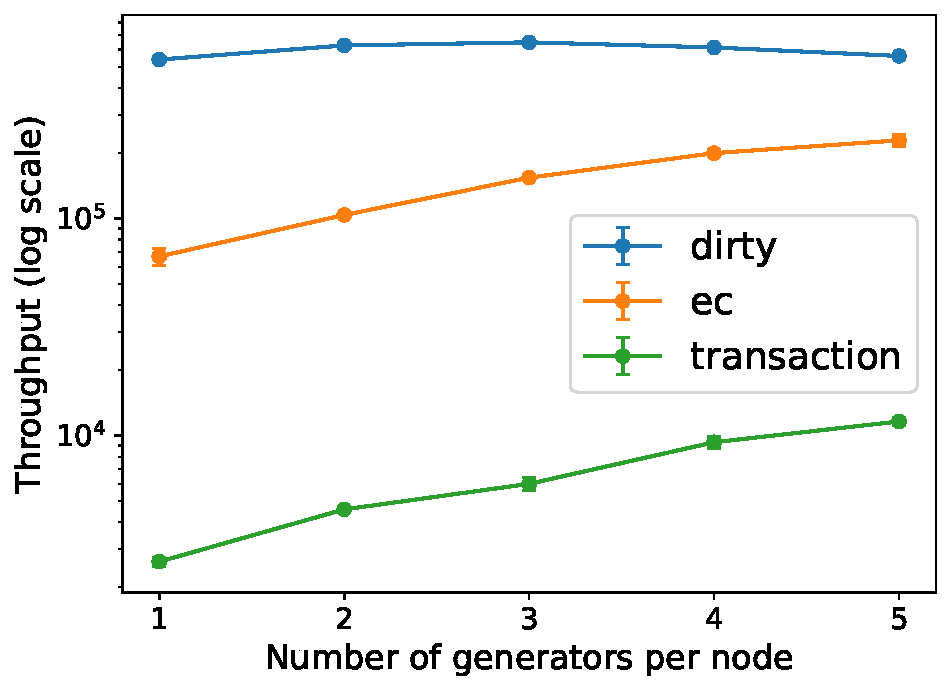
\includegraphics[width=\columnwidth]{figures/tp_generators_caelum.pdf}
    \caption{Throughput}
    \label{fig:tp generators caelum}
  \end{subfigure}
  \begin{subfigure}[t]{0.49\columnwidth}
    \centering
    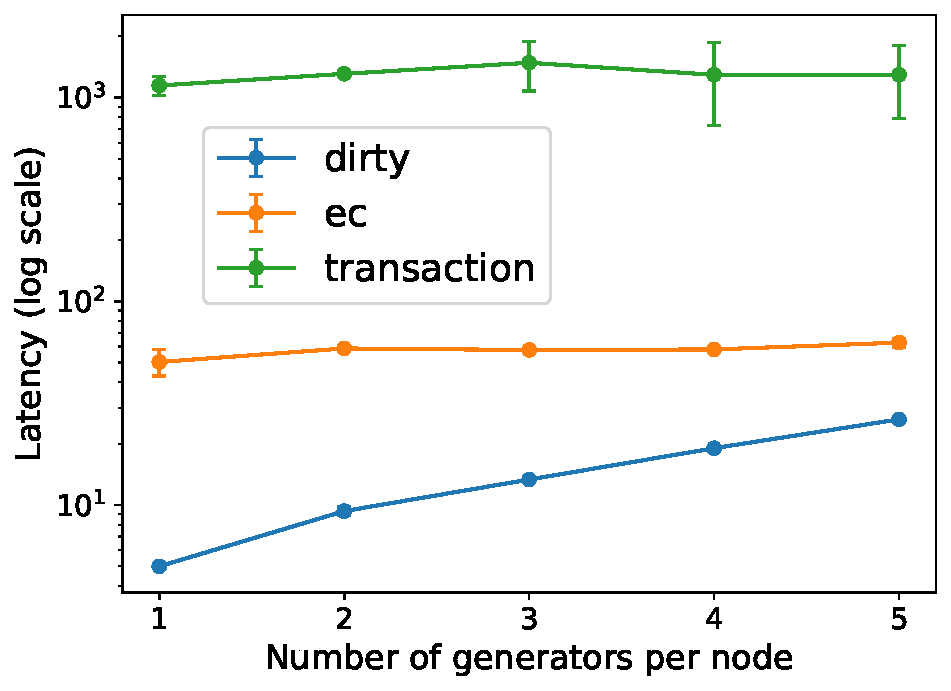
\includegraphics[width=\columnwidth]{figures/lat_generators_caelum.pdf}
    \caption{Latency}
    \label{fig:lat generators caelum}
  \end{subfigure}
  \caption{Throughput and latency against the number of generators. More generators
  generally bring higher throughput and latency.}
  \label{fig:generators caelum}
\end{figure}


\subsection{Cluster size} \label{subsec:eval cluster size}

This section evaluates the throughput and latency against the number of nodes in the 
Mnesia cluster. Based on the original design of Mnesia (\cref{sec:bg mnesia}), 
the number of nodes used in a cluster generally does not exceed ten~\cite{hebert2013LYSE}.
\Cref{fig:tp nodes fixgen caelum} and \cref{fig:lat nodes fixgen caelum} show the 
throughput and latency change with respect to
the number of nodes, with a fixed number (2) of generators. We observe that
the throughput decreases and the latency increases as the number of nodes increases,
suggesting that adding more nodes inevitably introduces overhead into the system,
e.g.\ more messages to send, and more data to process. Keeping the number of
generators the same means we keep the total amount of client requests
the same but add duplicate work by adding more replicas, therefore the system
experiences more overhead.

\begin{figure}[htp]
  \centering
  \begin{subfigure}[t]{0.49\columnwidth}
    \centering
    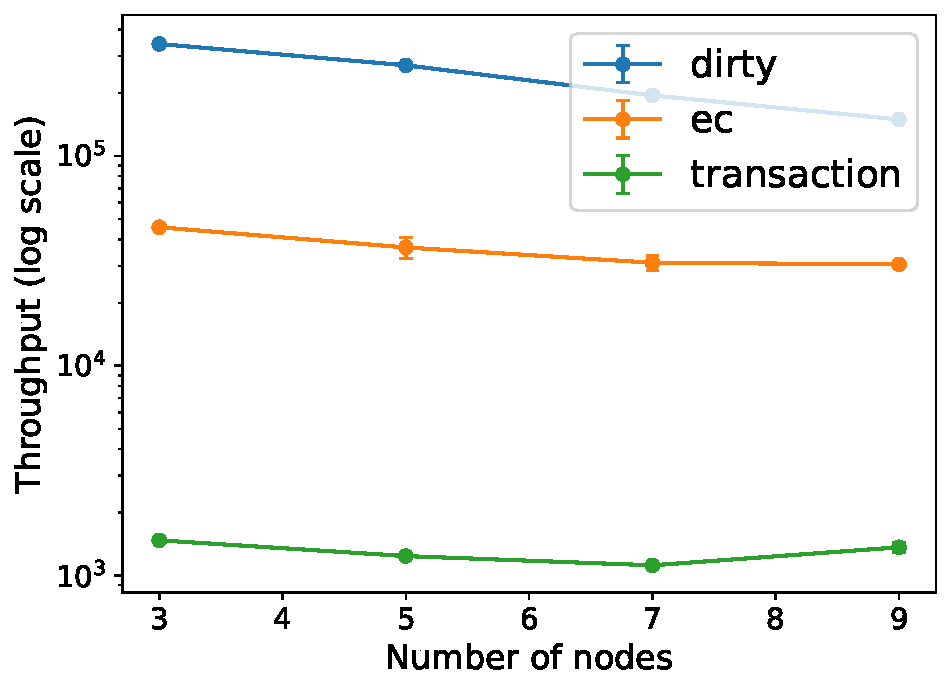
\includegraphics[width=\columnwidth]{figures/tp_nodes_fixgen_caelum.pdf}
    \caption{Throughput with a fixed number of generators.}
    \label{fig:tp nodes fixgen caelum}
  \end{subfigure}
  \begin{subfigure}[t]{0.49\columnwidth}
    \centering
    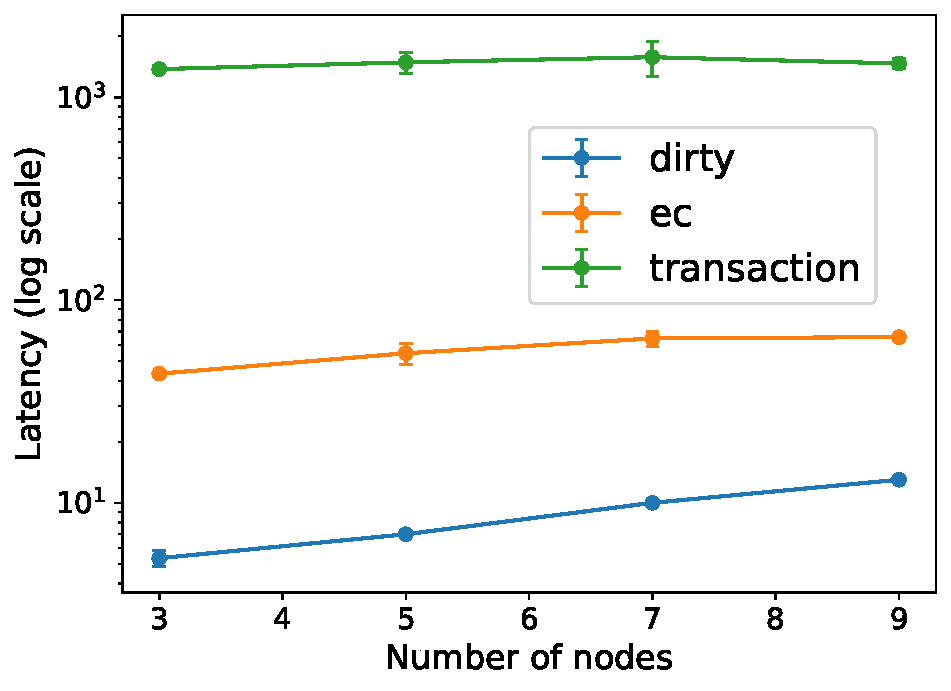
\includegraphics[width=\columnwidth]{figures/lat_nodes_fixgen_caelum.pdf}
    \caption{Latency with a fixed number of generators.}
    \label{fig:lat nodes fixgen caelum}
  \end{subfigure}

  \centering
  \begin{subfigure}[t]{0.49\columnwidth}
    \centering
    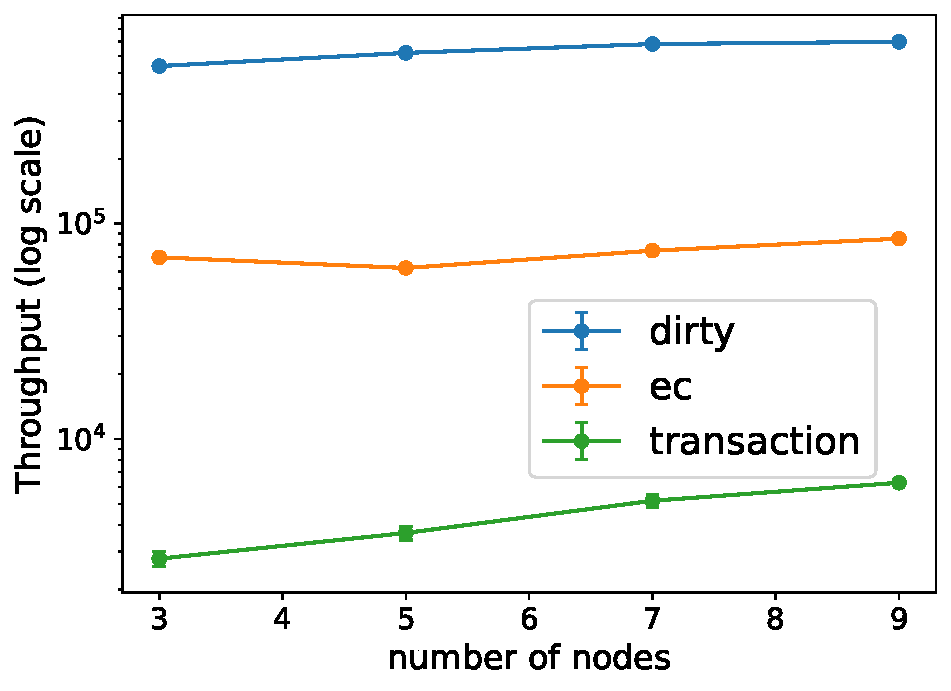
\includegraphics[width=\columnwidth]{figures/tp_nodes_caelum.pdf}
    \caption{Throughput with varying number of generators.}
    \label{fig:tp nodes caelum}
  \end{subfigure}
    \begin{subfigure}[t]{0.49\columnwidth}
    \centering
    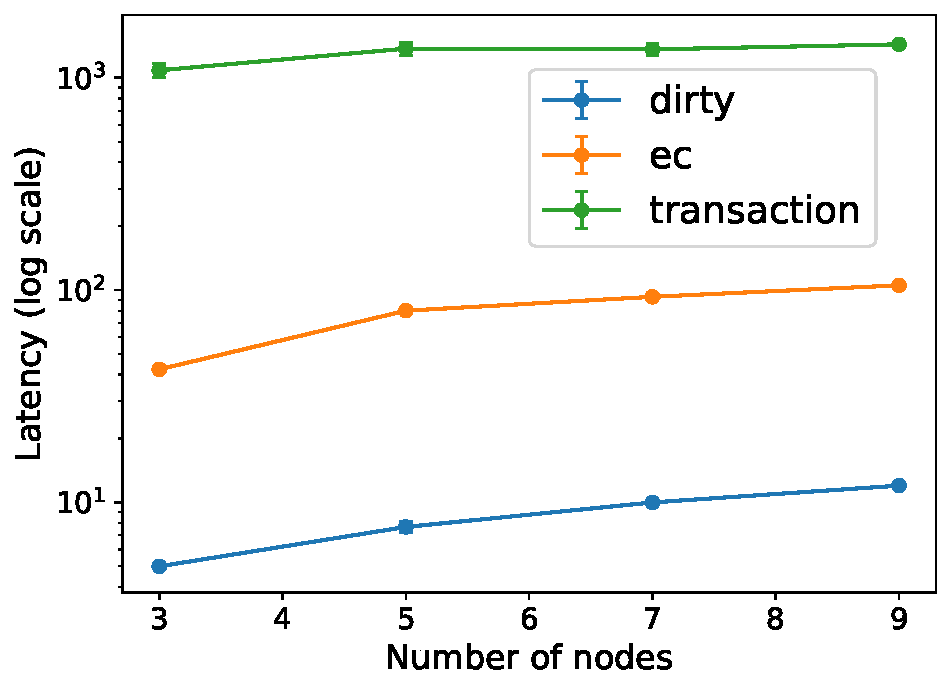
\includegraphics[width=\columnwidth]{figures/lat_nodes_caelum.pdf}
    \caption{Latency with varying number of generators.}
    \label{fig:lat nodes caelum}
  \end{subfigure}
  \caption{Throughput and latency against the number of nodes with fixed or
  varying number of generators. Adding replicas increases the overhead, but can be
  reduced by adding generators and increasing parallelism.}
  \label{fig:nodes caelum}

\end{figure}


However, we could also increase the number of generators as we have more replicas,
which is generally what happens in a real deployment as the number of nodes in a cluster 
of replicated machines increases.
\Cref{fig:tp nodes caelum} and~\cref{fig:lat nodes caelum} show the throughput and 
latency as the number of generators increases linearly with the number of nodes.
For all three operations, throughput increase is observed. Dirty operations' throughput
saturates at about 7 nodes, when the message queue backlog starts to become the
bottleneck. In terms of latency, there is an increase in all three. \acrshort{ec} 
operations demonstrate around \(13\)x higher throughput than transactions when 
there are nine nodes.

A higher replication factor often implies extra work for the system, thus resulting
in lower throughput and higher latency. However, we could offset this with more
clients and hence more parallelism. The overall effect is an increasing
throughput as the number of nodes increases, albeit with an inevitable sacrifice 
in latency. For \acrshort{ec} operations, this is approximately \qty{60}{\micro\second}.
This property is present in all three access contexts.


\subsection{Workload types} \label{subsec:eval workload types}

\Cref{fig:workload caelum} compares the throughput and latency of three access
contexts against different workloads. Dirty operations are about
\(50\)x better than transactions, while \acrshort{ec} operations lie between 
them (again), with about \(10\)x higher throughput than transactions.

Note that if the read percentage is \(100\%\), i.e.\ a read-only workload, the
transaction gets close to or even surpasses the performance of \acrshort{ec}
operations. This is due to an optimisation done in the benchmark where it
uses a synchronous dirty operation for reading data rather than a full
two-phase commit, which removes the cost of locking, and multi-round communication
time. It is even faster than \acrshort{ec} operations as it does not need to
go through the causal broadcast layer and the processing logic of an \acrshort{awset}.

\begin{figure}[htp]
  \centering
  \begin{subfigure}[t]{0.49\columnwidth}
    \centering
    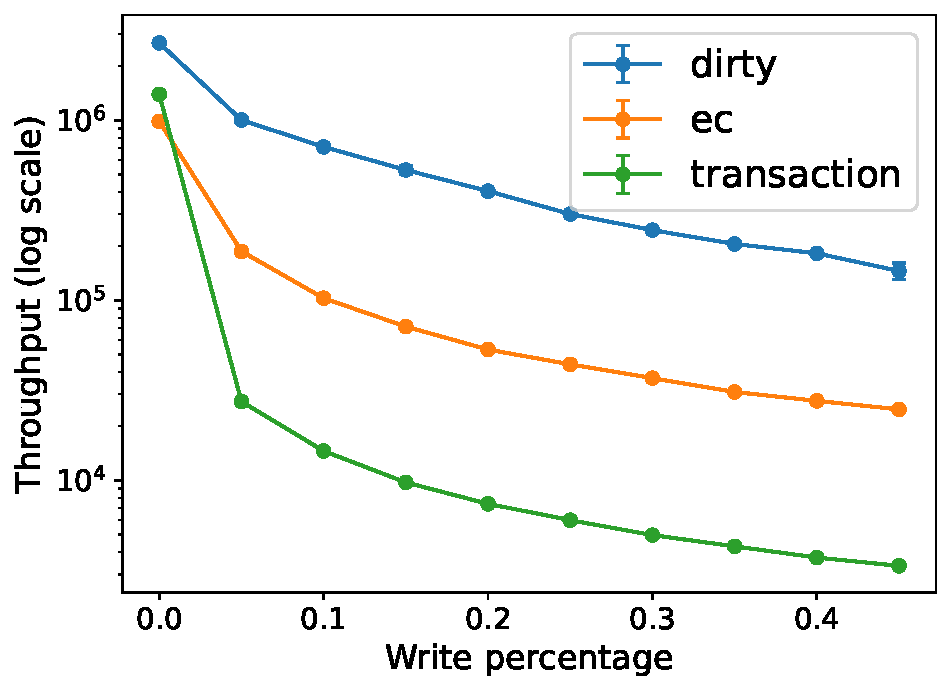
\includegraphics[width=\columnwidth]{figures/tp_rw_caelum.pdf}
    \caption{Throughput}
    \label{fig:tp workload caelum}
  \end{subfigure}
  \begin{subfigure}[t]{0.49\columnwidth}
    \centering
    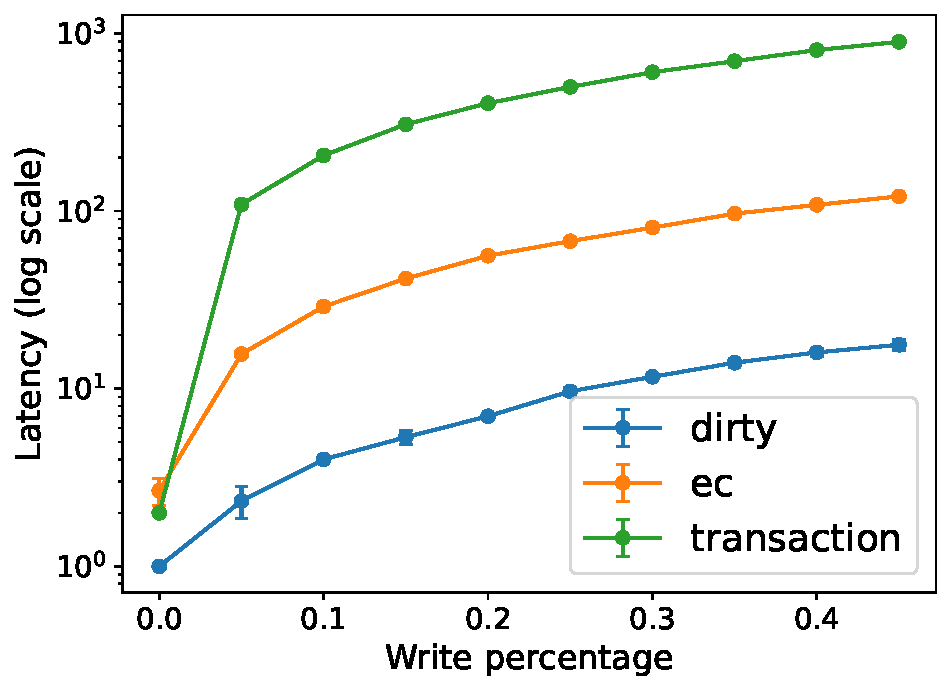
\includegraphics[width=\columnwidth]{figures/lat_rw_caelum.pdf}
    \caption{Latency}
    \label{fig:lat workload caelum}
  \end{subfigure}
  \caption{Throughput and latency against different workload types. Read-heavy
  workloads are faster than write-heavy ones in all three cases.}
  \label{fig:workload caelum}
\end{figure}

Write-intensive workloads are generally slower than read-intensive ones, since
writes need to involve all replicas in the cluster, while reads can be done
locally (if the data is present on the local node, which is the case in this
benchmark). This trend is, again, true for all three contexts. As long as the workload
is not read-only, \acrshort{ec} operations performs better than transactions.


\subsection{Table size} \label{subsec:eval table size}

\Cref{fig:table caelum} shows the change in throughput and latency as we vary
the size of the subscriber table. There are five tables in total in this benchmark, 
and the subscriber table stores the data for users
subscribing to a service, which is the most frequently changed and the largest one 
among all five tables. Therefore I choose to vary the 
subscriber table size during the initial table population.

A larger table generally makes it slower to read/write data, which affects
dirty operations but has less impact on transactions and
\acrshort{ec} operations. Similar to the behaviour in~\cref{subsec:eval generator number}, 
the low-latency dirty operations are more sensitive to even small changes in
the latency of each operation, and exhibits a larger increase in latency.


\begin{figure}[htp]
  \centering
  \begin{subfigure}[t]{0.49\columnwidth}
    \centering
    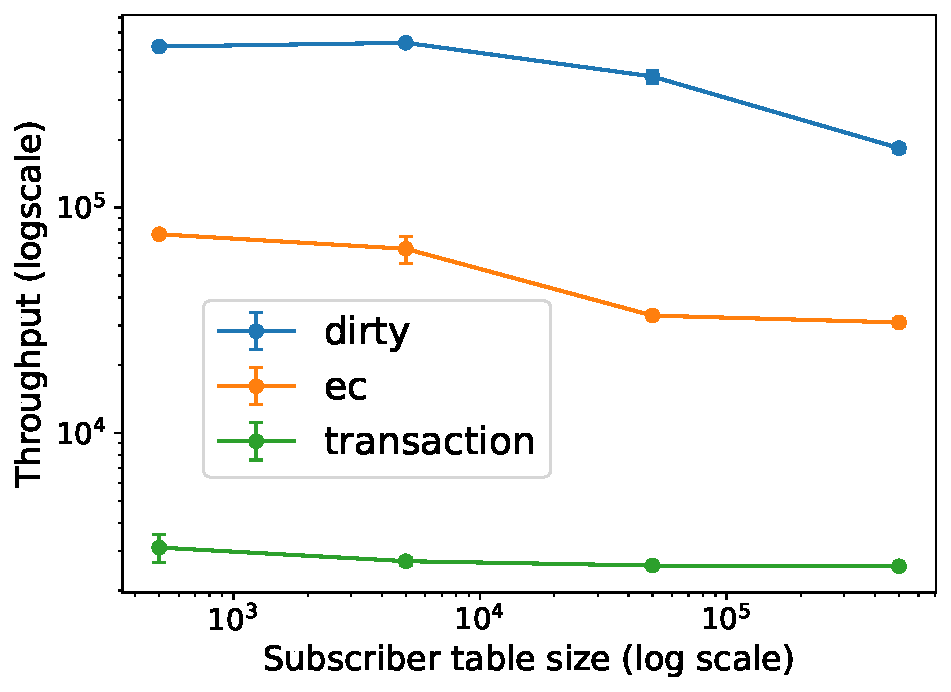
\includegraphics[width=\columnwidth]{figures/tp_table_caelum.pdf}
    \caption{Throughput}
    \label{fig:tp table caelum}
  \end{subfigure}
  \begin{subfigure}[t]{0.49\columnwidth}
    \centering
    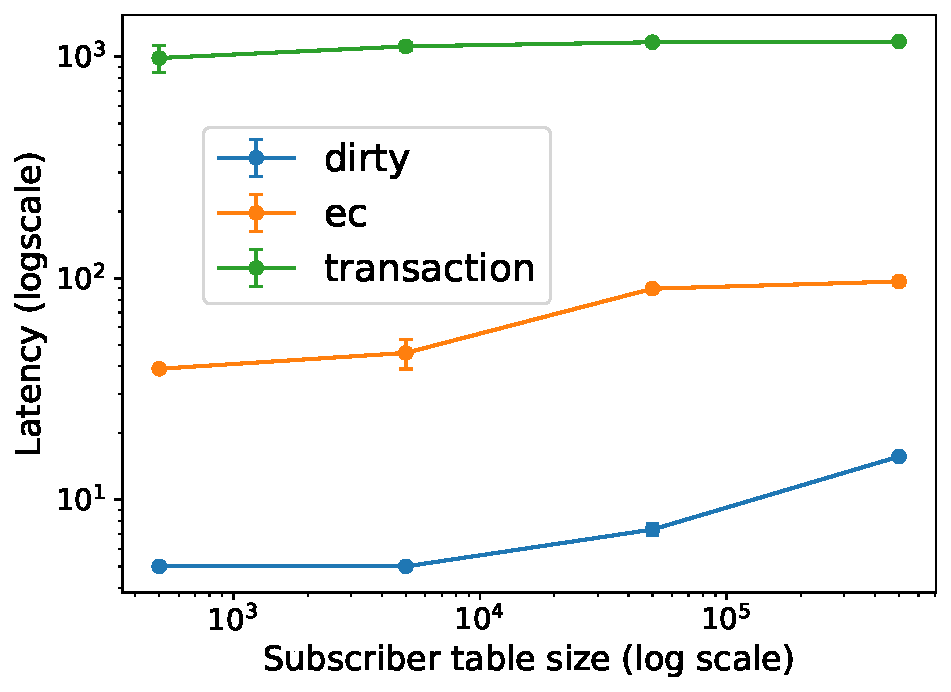
\includegraphics[width=\columnwidth]{figures/lat_table_caelum.pdf}
    \caption{Latency}
    \label{fig:lat table caelum}
  \end{subfigure}
  \caption{Throughput and latency against table size. Dirty operations are affected
  the most.}
  \label{fig:table caelum}
\end{figure}

Table size's impact on the performance of Hypermnesia mainly comes from the
extra time in accessing elements of a larger table. For \acrshort{ec} operations,
the extra overhead of periodic cleaning of timestamps could also play a 
role (\cref{subsec:impl causal stability}). However, this overhead 
is still acceptable as \acrshort{ec}
operations still have about \(25\)x higher throughput than transactions.

\subsection{Other databases} \label{subsec:eval other db}

Hypermnesia is also compared against two other databases to give a rough idea of its
relative throughput and latency, as discussed in~\cref{sec:eval benchmarks}. 
\Cref{fig:tp workload all} and \cref{fig:lat workload all}
shows the results of this experiments. We observe that Hypermnesia's throughput greatly
exceeds other two databases by more than ten times. Although we stress that (Hyper)mnesia
is an embedded database and such has quite different use cases and tradeoffs from the
other two.

\begin{figure}[htp]
    \centering
    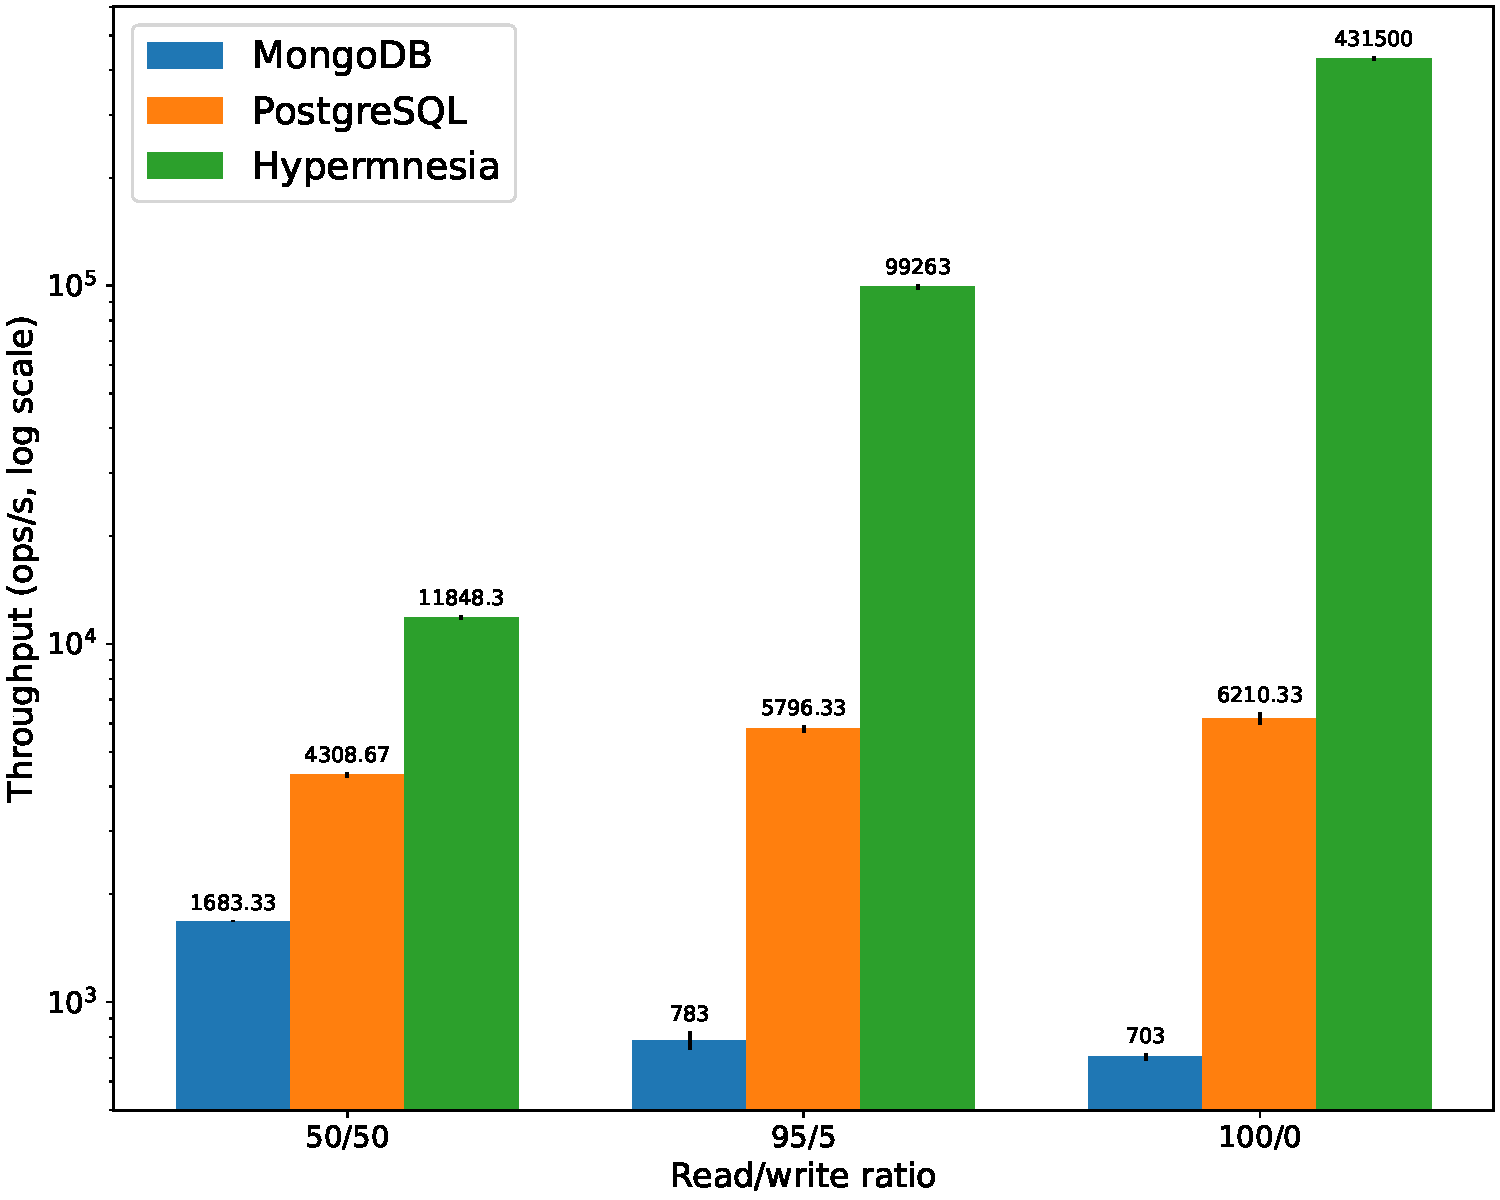
\includegraphics[width=0.96\columnwidth]{figures/tp_workload_all.pdf}
    \caption{Throughput}
  \caption{Throughput of different workloads, compared across MongoDB,
  PostgreSQL and Hypermnesia.}
  \label{fig:tp workload all}
\end{figure}


\begin{figure}[htp]
  \centering
  \begin{subfigure}[t]{0.48\columnwidth}
    \centering
    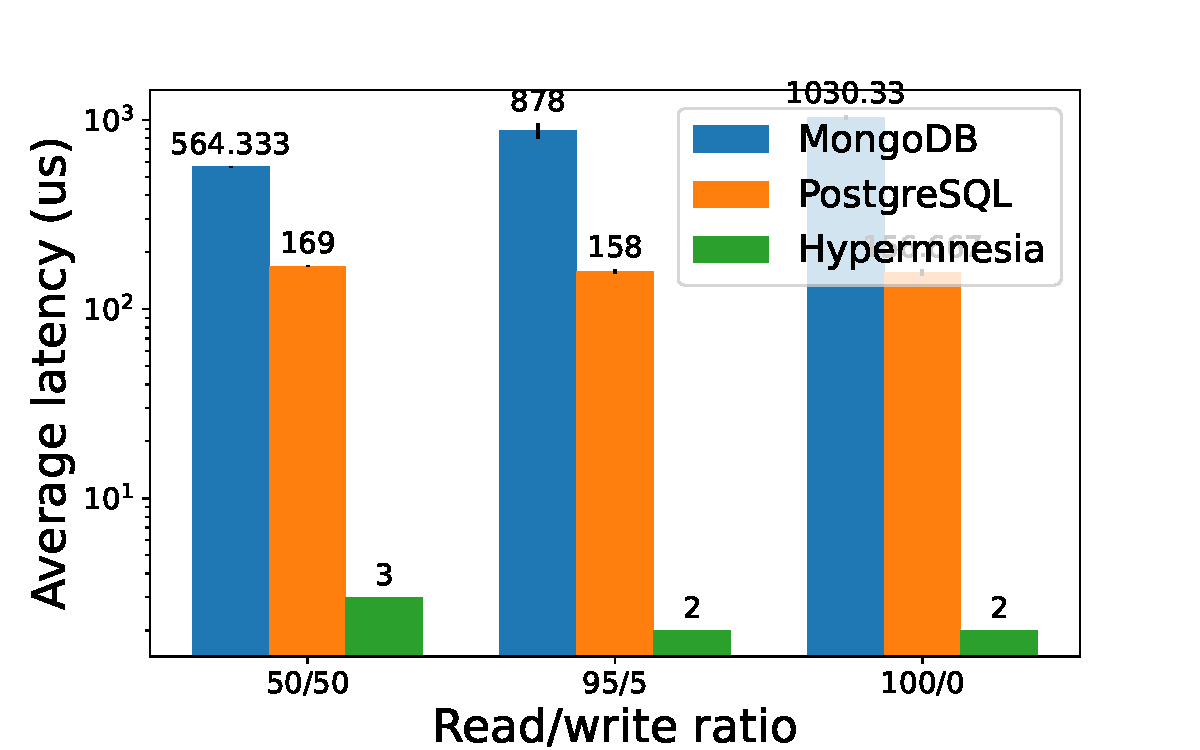
\includegraphics[width=\columnwidth]{figures/lat_workload_read_all.pdf}
    \caption{Read latency}
    \label{fig:tp workload read all}
  \end{subfigure}
  \begin{subfigure}[t]{0.48\columnwidth}
    \centering
    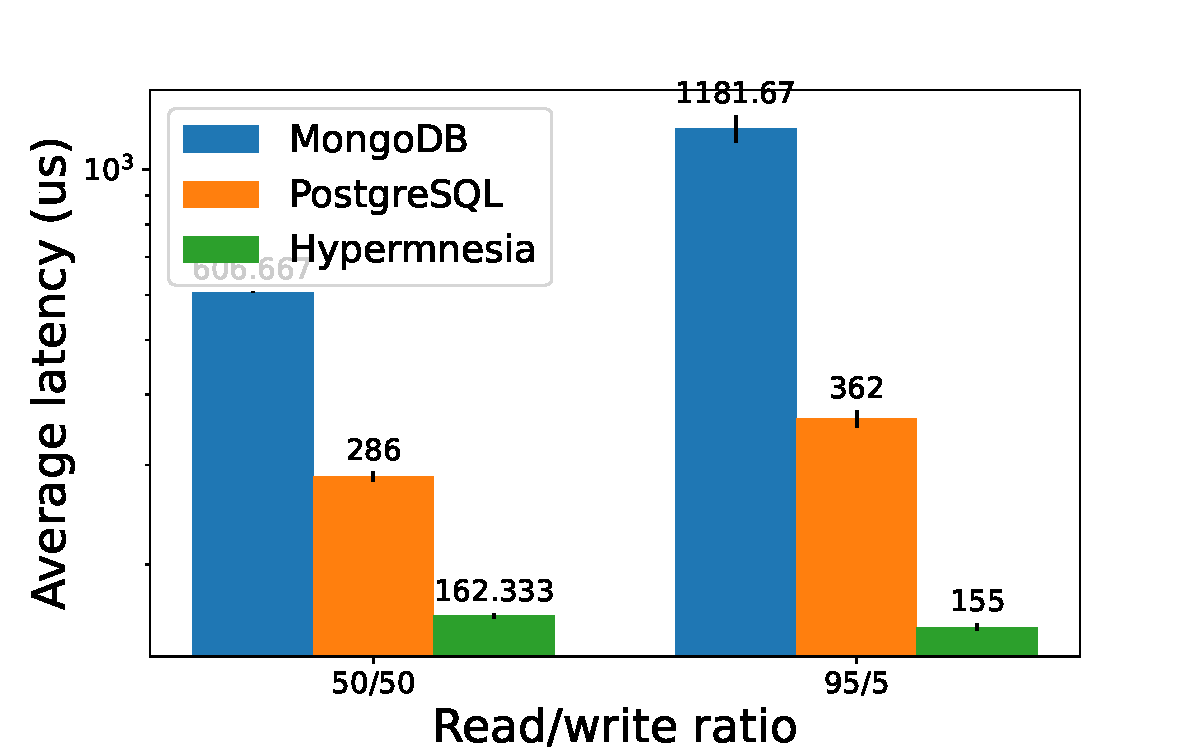
\includegraphics[width=\columnwidth]{figures/lat_workload_write_all.pdf}
    \caption{Write latency}
    \label{fig:lat workload write all}
  \end{subfigure}
  \caption{Latency of different workloads, compared across MongoDB,
  PostgreSQL and Hypermnesia.}
  \label{fig:lat workload all}
\end{figure}


\subsection{Space overhead} \label{sec:eval space}

This section evaluates the space overhead of Hypermnesia. Generally speaking,
\acrshortpl{crdt} rely heavily on metadata to keep track of the history of
operations and hence has a large overhead in its space usage~\cite{bauwens2019crdtmemory}. 
In the case of implementing a pure \acrshort{awset}, the primary
metadata associated with each element is the vector clock timestamp, which
grows linearly with the number of nodes in the cluster, although
garbage collection is implemented to reduce its impact (\cref{sec:impl pawset}).

\Cref{fig:space overhead populate} shows the pure op-based set's overhead
compared to the default set in Mnesia. The overhead grows linearly with respect
to the number of nodes as expected. Note that this is a static process, i.e.\ each
time the populator will put the same number of elements into the set, therefore
the lines are perfectly straight with no variance.
\Cref{fig:space overhead runtime} shows the
overhead after running the benchmark. This is a dynamic process during which
the causal stability optimisation is applied, but not in the previous
figure (we discuss the reason below). Observe that the causal stability optimisation
is able to reduce the overhead by up to \(30\%\).

\begin{figure}[htp]
  \centering
  \begin{subfigure}[t]{0.49\columnwidth}
    \centering
    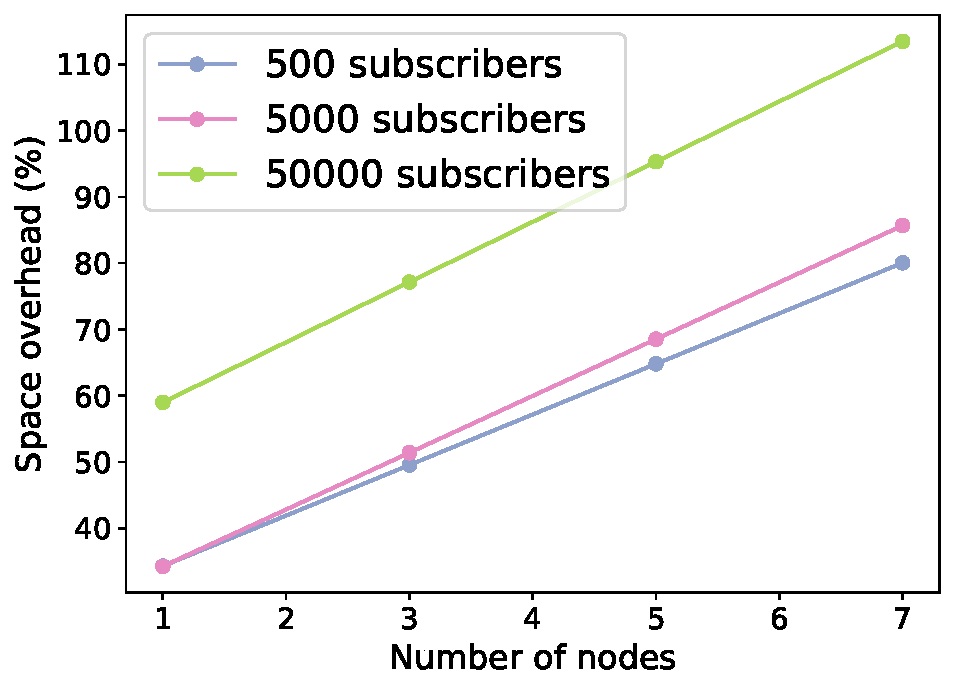
\includegraphics[width=\columnwidth]{figures/space_overhead_populate.pdf}
    \caption{Space overhead after populating the table.}
    \label{fig:space overhead populate}
  \end{subfigure}
  \begin{subfigure}[t]{0.49\columnwidth}
    \centering
    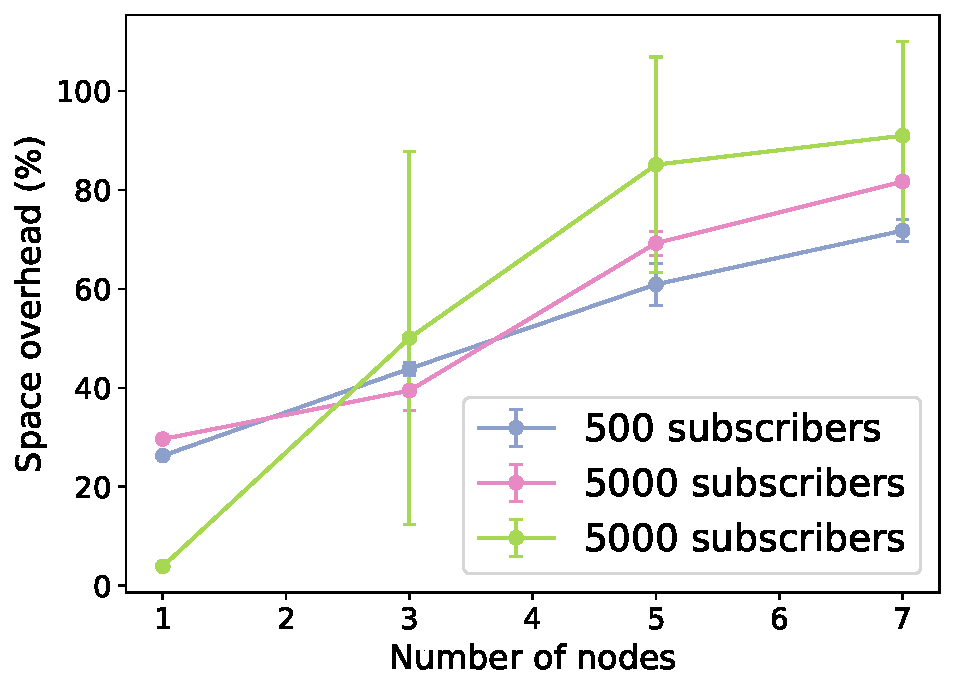
\includegraphics[width=\columnwidth]{figures/space_overhead_runtime.pdf}
    \caption{Space overhead after running the benchmark.}
    \label{fig:space overhead runtime}
  \end{subfigure}
  \caption{Space overhead. The number of subscribers represents the size of the
  table.}

\end{figure}


Despite space optimisations, the space overhead is still relatively large, especially 
when the number of nodes exceeds five. There are several reasons for this:

\begin{itemize}
  \item The underlying implementation of the \acrshort{polog} is a 
  set-like structure rather than a partially ordered 
  log (\cref{subsec:impl practical}). This complicates the implementation of
  causal stability optimisation as it is now harder to find all elements with
  a timestamp smaller than the stable one.
  \item The causal stability optimisation relies on nodes continuously receiving 
  updates from other nodes to determine timestamp stability. This is not always
  possible since it is common for a node to only receive messages from 
  others (maybe no client sends requests to it).
  This is why the optimisation is not applied in the
  population phase. \citet{bauwens2019crdtmemory} made a similar observation and 
  proposed a solution based on an eager collection of metadata.
\end{itemize}

Memory management has been an important issue in \acrshort{crdt} research but has
yet to attract much attention~\cite{bauwens2019crdtmemory}. The current optimisation
using causal stability is less effective than one would hope for. In a typical
setup of three nodes, the extra space needed is around \(30\)--\(40\%\). For
this reason, Hypermnesia is limited to relatively small clusters, but this is acceptable
since Mnesia is designed for small clusters in the first place~\cite{hebert2013LYSE}.
We discuss more on how to optimise the space overhead of the 
Set \acrshort{crdt} in~\cref{sec:concl future}.


\subsection{Fault tolerance} \label{sec:eval fault tolerance}

\Cref{sec:impl fault tolerance} discusses how Mnesia and Hypermnesia respond 
to network partitions. In this section, we evaluate Hypermnesia against these two 
situations to answer the research question~\cref{itm:question ec conflict} 
in~\cref{sec:intro motivation}.

\paragraph{Communication failure} \label{para:eval comm failure}

Mnesia does not handle communication failure by default and asks
application developers to resolve conflicts. Hypermnesia buffers operations during
the partition until it recovers (\cref{fig:hypermnesia comm failure}). It then
sends the buffered message and resolves conflicts automatically.

\paragraph{Transient failure} \label{para:eval transient failure}

As discussed in~\cref{subsec:bg cap}, during a transient failure,
transactions stall until the partition heals. We measure this effect by
examining the throughput change in a simulated network partition, as shown
in~\cref{fig:tp time partition}. \Cref{fig:tp time without partition} shows how the 
throughput changes through time, which is
relatively stable when there is no partition. On the other 
hand, \cref{fig:tp time with partition}
shows the throughput when there is a (simulated) network partition, lasting around
10 seconds. Dirty and \acrshort{ec} operations remain about the same, but transaction
throughput drops down to zero during the partition period. This is expected since
the two-phase commit protocol requires a reply from \emph{all} participating nodes.

\begin{figure}[htp]
  \centering
  \begin{subfigure}[t]{0.49\columnwidth}
    \centering
    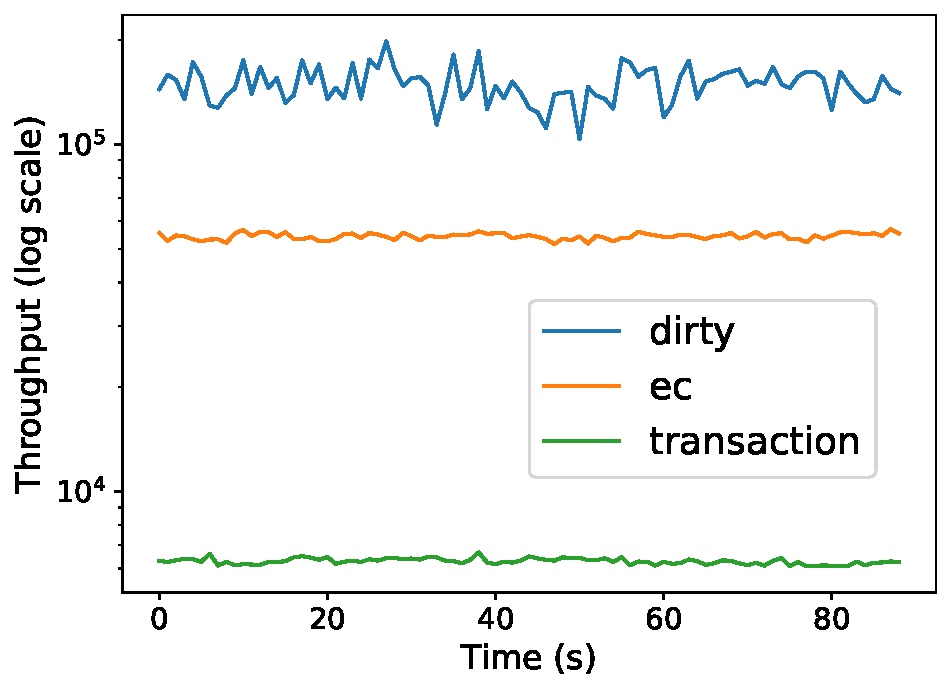
\includegraphics[width=\columnwidth]{figures/tp_time_single.pdf} 
    \caption{No partition.}
    \label{fig:tp time without partition}
  \end{subfigure}
  \begin{subfigure}[t]{0.49\columnwidth}
    \centering
    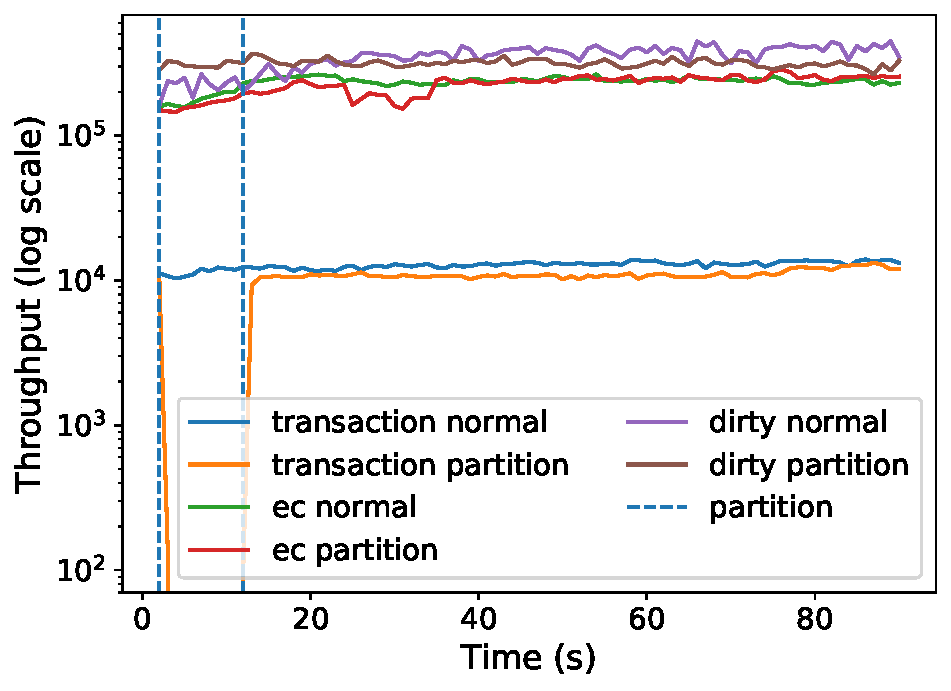
\includegraphics[width=\columnwidth]{figures/tp_time_partition.pdf} 
    \caption{A partition of 10 seconds, dashed lines indicate the start and
    end of the partition.}
    \label{fig:tp time with partition}
  \end{subfigure}
  \caption{Throughput changes against time. Network partition affects the transaction
  throughput but not dirty and \acrshort{ec} throughputs.}
  \label{fig:tp time partition}
\end{figure}

In summary, Hypermnesia adds fault tolerance to Mnesia in the presence of network partitions:
\begin{enumerate*}
  \item automatic conflict resolution after a communication failure;
  \item nodes remain available during transient failure, with guaranteed convergence
  when the partition heals. 
\end{enumerate*}

\subsection{APIs and refactoring} \label{sec:eval api}

This section attempts to answer the research question~\cref{itm:question ec refactor} 
concerning refactoring. First, a summary of the code changes is given for Hypermnesia, 
followed by experimental modifications of real-world applications to demonstrate 
Hypermnesia's usability.

\Cref{lst:ec api comparison} shows the code changes needed from transactions/dirty
operations (first two columns) to \acrshort{ec} operations (last column).
Note that refactoring is often just one line of change. Another change 
is the \texttt{type} option while creating
a Mnesia table, as shown in~\cref{lst:hypermnesia type decl}. And that is all
the change needed to use the new API\@. 

\begin{listing}[htp]
  \begin{sublisting}[t]{0.48\columnwidth}
    \begin{minted}[frame=lines]{erlang}
      mnesia:activity(transaction, 
      fun () -> 
        mnesia:write(tab, tup),
        mnesia:read(tab, key)
      end).
    \end{minted}
    \caption{transactions with \texttt{activity/2}.}
  \end{sublisting}
  \begin{sublisting}[t]{0.48\columnwidth}
    \begin{minted}[frame=lines]{erlang}
      mnesia:activity(async_dirty, 
      fun () -> 
        mnesia:write(tab,tup),
        mnesia:read(tab,key)
      end).
    \end{minted}
    \caption{dirty with \texttt{activity/2}.}
  \end{sublisting}
  
  \begin{sublisting}[t]{\columnwidth}
    \begin{minted}[frame=lines]{erlang}
      mnesia:activity(async_ec, 
      fun () -> 
        mnesia:write(tab,tup),
        mnesia:read(tab,key)
      end).
    \end{minted}
    \caption{\acrshort{ec} operations with \texttt{activity/2}}
  \end{sublisting}
  \begin{sublisting}[t]{0.48\columnwidth}
    \begin{minted}[frame=lines]{erlang}
      mnesia:transaction(
      fun () -> 
        mnesia:write(tab,tup),
        mnesia:read(tab,key)
      end).
    \end{minted}
    \caption{transactions with \texttt{transaction/1}}
  \end{sublisting}
  \begin{sublisting}[t]{0.48\columnwidth}
    \begin{minted}[frame=lines]{erlang}
      mnesia:async_dirty(
      fun () -> 
        mnesia:write(tab,tup),
        mnesia:read(tab,key)
      end).
    \end{minted}
  \caption{dirty with \texttt{async\_dirty/1}}
  \end{sublisting}
  
  \begin{sublisting}[t]{\columnwidth}
      \begin{minted}[frame=lines]{erlang}
        mnesia:async_ec(
        fun () -> 
          mnesia:write(tab,tup),
          mnesia:read(tab,key)
        end).
      \end{minted}
    \caption{\acrshort{ec} operations with \texttt{async\_ec/1}}
  \end{sublisting}
  \caption{Changing from transaction or dirty operations to \acrshort{ec} operations.}
  \label{lst:ec api comparison}
\end{listing}


\begin{listing}[htp]
  \centering 
  \begin{sublisting}[t]{\columnwidth}
    \centering
    \begin{minted}[frame=lines]{erlang}
      ejabberd_mnesia:create(?MODULE, oauth_client, [{disc_copies, [node()]},
       {attributes, record_info(fields, oauth_client)}, {type, set}]).
    \end{minted}
    \caption{Original code creating a Mnesia table, using a set data structure.}
  \end{sublisting}
  
  \begin{sublisting}[t]{\columnwidth}
    \centering
    \begin{minted}[frame=lines]{erlang}
      ejabberd_mnesia:create(?MODULE, oauth_client, [{disc_copies, [node()]},
       {attributes, record_info(fields, oauth_client)}, {type, pawset}]).
    \end{minted}
    \caption{New code using the pure \acrshort{awset} (pawset).}
  \end{sublisting} 
  \caption{Adding a type declaration when creating a Mnesia table. Code excerpt
  modified from ejabberd~\cite{processone2023ejabberd}.}
  \label{lst:hypermnesia type decl}
\end{listing}

The second step is to apply the refactoring described above in actual production
codebases such as RabbitMQ~\cite{vmware2023rabbitmq} and 
ejabberd~\cite{processone2023ejabberd}, and run the regression test suites against
such changes. To be more cautious while refactoring, most changes
are from asynchronous dirty operations to asynchronous \acrshort{ec} operations. 
Hypermnesia successfully passes the test suites of both applications with little
effort in changing the source code.

It is worth noting that this is not a formal usability study of the new API.
A more rigorous study requires much more extensive testing and understanding
of the project codebases, which requires lots of engineering effort and is beyond
the scope of this project. Nevertheless, we believe this evaluation is a first
step towards making Hypermnesia more usable and production-ready.


% \subsection{Summary}

% In this chapter, we evaluated Hypermnesia against the research questions
% of this project (\cref{sec:intro motivation}). The results show that Hypermnesia can
% produce correct results in spite of network delays (\cref{sec:eval correctness}),
% and partitions (\cref{sec:eval fault tolerance}), thus demonstrating the possibility
% of \acrlong{ec} in Mnesia and its role in automatic conflict 
% resolution (\cref{itm:question ec possible,itm:question ec conflict}).
% Furthermore, benchmarking results show that \acrshort{ec} operations can achieve
% approximately \(10\)--\(20\)x better throughput and lower latency than transactions, 
% and its performance can get close to dirty operations (recall that dirty operations 
% are much faster than transactions in Mnesia from~\cref{subsec:mnesia access contexts}) 
% when increasing the scale of the experiment (\cref{sec:eval benchmarks}).
% This makes \acrshort{ec} operations competitive for real-world applications
% (\cref{itm:question ec overhead}).
% Finally, \cref{sec:eval api} evaluates the usability of the new 
% API (\cref{itm:question ec refactor}) and shows that
% Hypermnesia's API enables minimum code refactoring for adoption in real-world
% projects.
